\section{Integration}
\label{sec:integration}

If the controller is implemented and tested, it's ready for \textsf{C} code generation (or \textsf{C++}, \textsf{Verilog} or \textsf{PLC}). Find the correct subsystem that acts as the controller, and build the model with the \verb!MATLAB! \texttt{Embedded} \verb!Coder!. In a large system, it is possible to generate separate source code implementations of different subsystems. Though the integration complexity increases, it can provide enhanced functionality, and excellent reusability.

\subsection{Structure of the Generated Code}

If during the code generation \emph{Compact code placement} was used, only four files are generated. Figure \ref{fig:rtw} shows the connection between these files. 

\begin{minipage}{0.45\linewidth}
	\begin{itemize}
		\item "system\_name".c
		\item "system\_name".h
		\item rtwtypes.h
		\item ert\_main.c
	\end{itemize}
\end{minipage}
\begin{minipage}{0.45\linewidth}
	\begin{figure}[H]
		\centering
		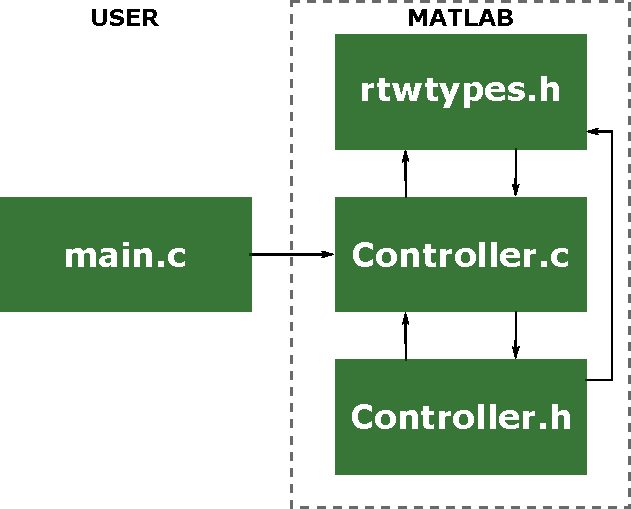
\includegraphics[width=0.8\linewidth]{img/rtw}
		\caption{Relationship of the generated files}
		\label{fig:rtw}
		\vspace{10pt}
	\end{figure}
\end{minipage}


In the following we assume that the name of the Controller block was "model". The functions of the system are defined in the \texttt{model.c} and \texttt{model.h} files. The \texttt{rtwtypes.h} contains the unique type definitions of the code. The \texttt{ert\_main.c} is an exemplary main function that demonstrates the use of the others.

\subsection{Using the Controller Source Code}

The generated source code is functionally equivalent to the \textsf{Simulink} model. A number of functions and variable structures are defined that implement an easy interface of control the module, and communication with the system is only possible through this unique interface provided by the generated code. The system can be initialized using the \emph{model\_initialize()} function. It sets the 0 time in the model, and the outputs assume their initial values. The inputs are handled by the \emph{model\_U} struct. It contains fields each corresponding to a system input, matching it's name and type. If the inputs are set, calling the \emph{model\_step()} function runs the model once, for the period of one time sample. The outputs are stored in a structure similar to the input storage, called \emph{model\_Y}.

\subsection{Deployment with FreeRTOS on STM32F4-Discovery Board}

As in many controlled processes, the timing of the controller program execution is crucial, as well as the processing of the \textsf{I/O} ports, converting the analogue signals and sending status information to the supervisor computer over a wireless connection. It can be implemented with integrated timer peripherals and interrupt sequences, but in case of a multi task system, the application of a \emph{Real Time Operating System} allows a more high-level approach. There are numerous implementations of this operating system family. We chose \textsf{FreeRTOS}, a popular open-source operating system in the industry, because of its detailed documentation and earlier work experiences with the operating system on \textsf{STM32F4-Discovery}. In addition, it provides useful features for application debugging.

\begin{figure}[H]
    \centering
    \includegraphics[width=0.7\linewidth]{img/integration}
    \caption{Connections between modules}
    \label{fig:integration}
\end{figure}

Figure \ref{fig:integration} illustrates the usage of the technologies. In our solution the \textsf{FreeRTOS} is responsible for the task scheduling, and provide a communication interface between the tasks. This way we can ensure that the sensor readings and the controller task are conducted with precise timing. Through the operating system direct communication with the \textsf{I/O} ports is simple, and it handles the processing of the optoelectronic and proximity sensor signals with the Analogue to Digital converters of the board.

Setting up the system requires the inclusion the \textsf{FreeRTOS} source files in the project and some additional low level drivers to read the sensors, and initialize the actuators. Once the Core system is ready, the generated source files are included and periodically called by a timer, and its input and output \emph{structs} are connected to the electronics through the low-level drivers.